\chapter{Low Rank Building Change Detection Method }
\label{chap:method}

\noindent
This chapter presents the methodological framework developed for \textbf{building change detection (BCD)} in very-high-resolution (VHR) satellite imagery. The central objective is to identify when and where man-made structures have appeared, disappeared, or undergone modifications between two acquisition periods. In this context, BCD is formulated as a \textit{bi-temporal semantic segmentation problem}, where the model receives two co-registered images of the same area and predicts a binary mask delineating the changed regions. 

\medskip
\noindent
Urban areas—particularly those of Latin America—pose unique challenges for BCD. Variability in rooftop materials, dense informal settlements, and frequent occlusions caused by shadows or clouds complicate the detection process. Moreover, imperfect co-registration between image pairs and the scarcity of accurately labeled data amplify uncertainty during model training. These challenges highlight the need for a method that is robust to spatial noise, efficient in computation, and capable of detecting subtle yet significant changes at the building scale.

\medskip
\noindent
To address these constraints, our approach integrates two complementary strategies. First, a \textbf{Siamese hierarchical Transformer architecture (ChangeFormer)} is adopted to capture spatial and temporal relationships across multi-scale features. Second, we enhance the Transformer encoder with a \textbf{Rank-Augmented Linear Attention (RALA)} mechanism, which reduces the quadratic complexity of conventional self-attention while preserving its global context modeling capabilities. This hybrid design allows the model to efficiently process VHR imagery and maintain sensitivity to both local edge details and large-scale urban transformations.

\medskip
\noindent
The overall workflow of the proposed method is illustrated in Figure~\ref{fig:method-flow}. It is structured in three main stages:  

\begin{enumerate}[label=(\arabic*)]
    \item \textbf{Preprocessing:} Includes data preparation steps such as image co-registration, normalization, and patch extraction to ensure consistent bi-temporal inputs.
    \item \textbf{Detection of Building Changes:} The core stage of the framework, where the RALA-enhanced ChangeFormer encoder extracts deep temporal representations, computes feature differences, and classifies pixels into \textit{change} or \textit{no change}.
    \item \textbf{Localization of Building Changes:} Post-processing and refinement are applied to obtain the final binary change mask, highlighting the precise spatial extent of detected changes.
\end{enumerate}

\begin{figure}[h!]
    \centering
    % Placeholder for the actual diagram; replace with the final vector illustration.
    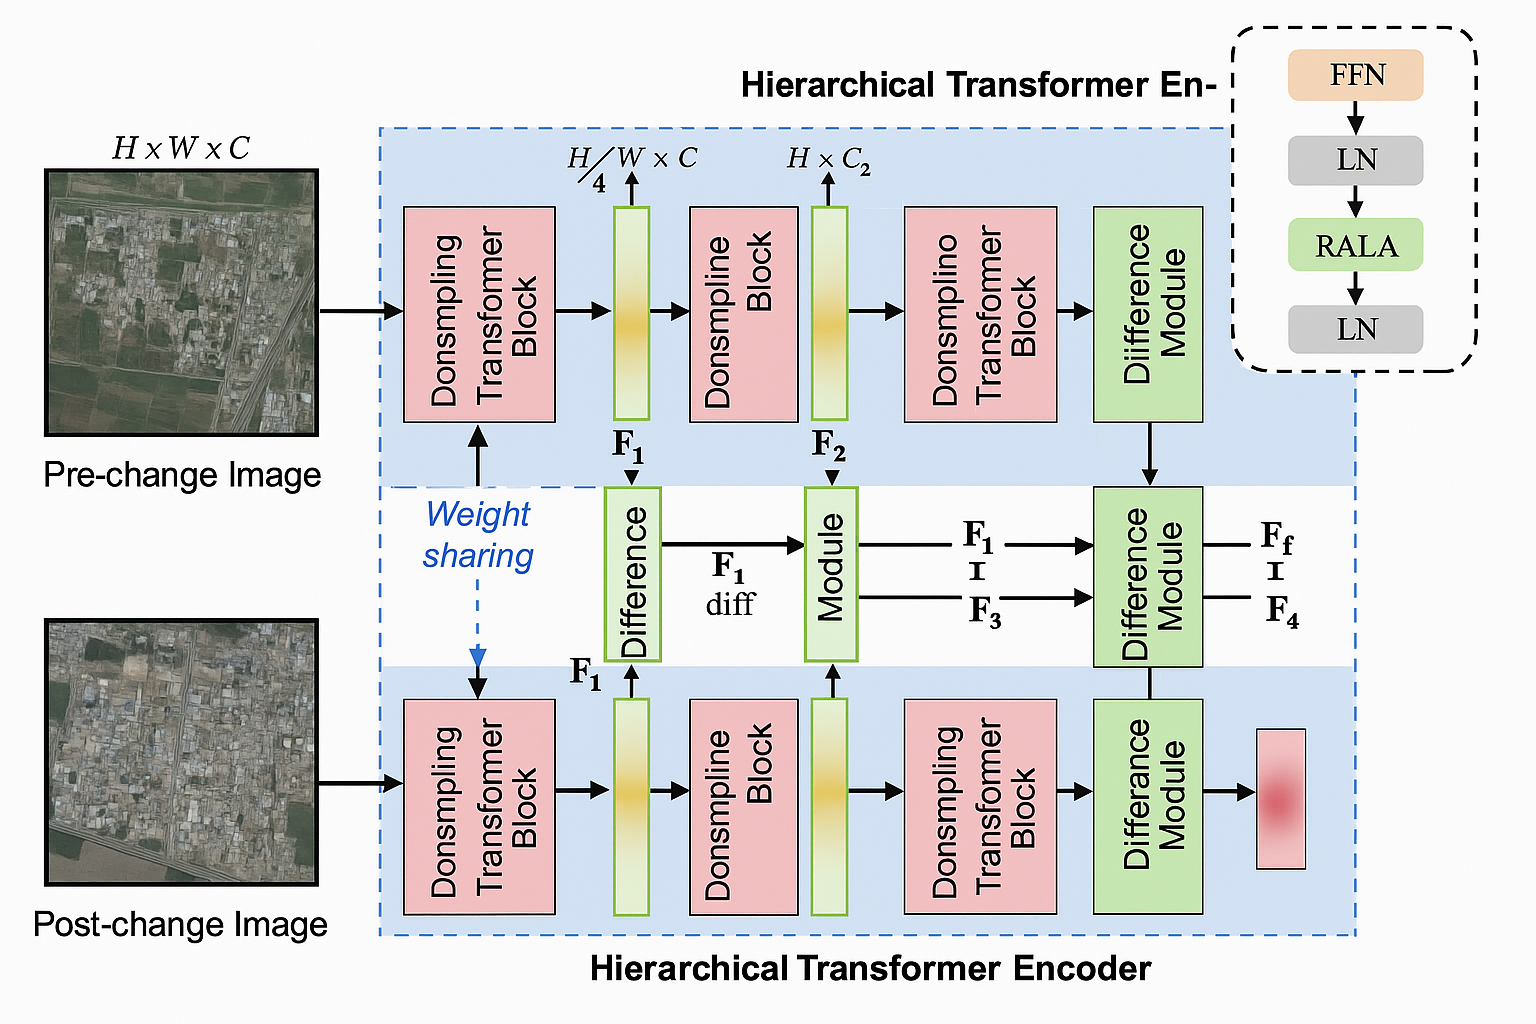
\includegraphics[width=0.8\textwidth]{graficos/workflow.png}
    \caption{\textbf{Overview of the proposed BCD pipeline.} 
    The process consists of three stages: (1) Preprocessing of bi-temporal images, (2) Detection of building changes using a RALA-enhanced Siamese Transformer encoder-decoder architecture, and (3) Localization of changes through post-processing and binary mask generation.}
    \label{fig:method-flow}
\end{figure}

\medskip
\noindent
The remainder of this chapter is organized as follows.  
Section~\ref{sec:problem-notation} defines the mathematical formulation of the problem.  
Section~\ref{sec:preprocessing} details the preprocessing steps applied to the datasets.  
Section~\ref{sec:detection} describes the detection stage, including the baseline \textit{ChangeFormer} architecture, the integration of the \textit{RALA} attention mechanism within its Transformer blocks, and the loss functions used for training.  
Section~\ref{sec:localization} explains the localization stage, outlining how binary masks are derived and refined to represent structural changes.  
Finally, Section~\ref{sec:final-considerations} summarizes the key methodological insights and discusses their implications for urban-scale change detection.

\section{Problem Definition}
\label{sec:problem-notation}

\noindent
The \textbf{building change detection (BCD)} task aims to identify structural modifications 
between two satellite images acquired at different times over the same geographic area. 
Formally, let the bi-temporal pair be:
\[
X = \{ I_t^1, I_t^2 \}, 
\qquad 
I_t^k \in \mathbb{R}^{H \times W \times C},
\quad k \in \{1,2\},
\]
where \(H\), \(W\), and \(C\) denote image height, width, and number of spectral channels.
The objective is to predict a binary change mask 
\(Y \in \{0,1\}^{H \times W}\), where \(Y_{i,j}=1\) indicates the presence of a building 
change between \(t_1\) (pre-event) and \(t_2\) (post-event).

\noindent
The model \(M_\theta\) learns a mapping:
\[
M_\theta: (I_t^1, I_t^2) \rightarrow \hat{Y},
\]
where \(\hat{Y}\) is a dense probability map estimating the likelihood of temporal change.
Training minimizes the discrepancy between \(Y\) and \(\hat{Y}\) through a hybrid loss:
\[
\min_{\theta} \mathcal{L}(Y, \hat{Y})
=
\mathcal{L}_{BCE}(Y, \hat{Y})
+
\lambda\, \mathcal{L}_{Dice}(Y, \hat{Y}),
\]
where \(\lambda=1.0\) balances pixel-wise precision and overlap-based consistency.

\paragraph{Training stage.}
Given a training set 
\(\mathcal{T}=\{(I_t^1, I_t^2, Y)\}_{i=1}^N\),
the network is optimized to approximate the true mapping 
\(f^*: (I_t^1, I_t^2) \mapsto Y\),
learning discriminative spatial–temporal patterns that characterize building additions, 
removals, or structural modifications.

\paragraph{Inference stage.}
For an unseen pair \((I_t^1, I_t^2)\), the model produces \(\hat{Y}\in [0,1]^{H\times W}\).
A threshold \(\tau=0.5\) yields the binary mask:
\[
Y_{\text{bin}}(i,j)=
\begin{cases}
1, & \hat{Y}(i,j)\ge\tau,\\[0.2em]
0, & \text{otherwise}.
\end{cases}
\]
The binary output highlights the spatial distribution of detected building changes and serves 
as the basis for the localization stage in Section~\ref{sec:localization}.



\section{Data Preprocessing}
\label{sec:preprocessing}

\noindent
Bi-temporal satellite images require consistent spatial and radiometric alignment before they 
can be processed by any deep model. The preprocessing stage ensures comparability between 
temporal acquisitions and converts raw remote sensing data into standardized patches suitable 
for Transformer-based architectures.

\paragraph{Image co-registration.}
Both images \(I_t^1\) and \(I_t^2\) are aligned to a common spatial reference through affine 
geometric corrections and cross-correlation refinement, preventing misalignment artefacts that 
could be incorrectly interpreted as changes.

\paragraph{Radiometric and geometric normalization.}
All spectral channels are normalized to the \([0,1]\) range:
\[
I' = \frac{I - \min(I)}{\max(I)-\min(I)}.
\]
Images are subsequently cropped or padded to ensure uniform dimensions across the dataset.

\paragraph{Patch extraction.}
Following the protocol in \cite{Bandara2022ChangeFormer}, each co-registered pair is divided 
into non-overlapping \(256\times256\) patches. Each patch yields a bi-temporal tensor of 
dimension \((256,256,2C)\). This strategy both expands the training set and fits within common 
GPU memory constraints.

\paragraph{Dataset preparation and augmentation.}
We adopt LEVIR-CD and DSIFN-CD for training and evaluation, using their official splits.
Random flips, rotations, brightness/contrast shifts, and Gaussian noise are applied to improve 
generalization.

\begin{figure}[h!]
    \centering
    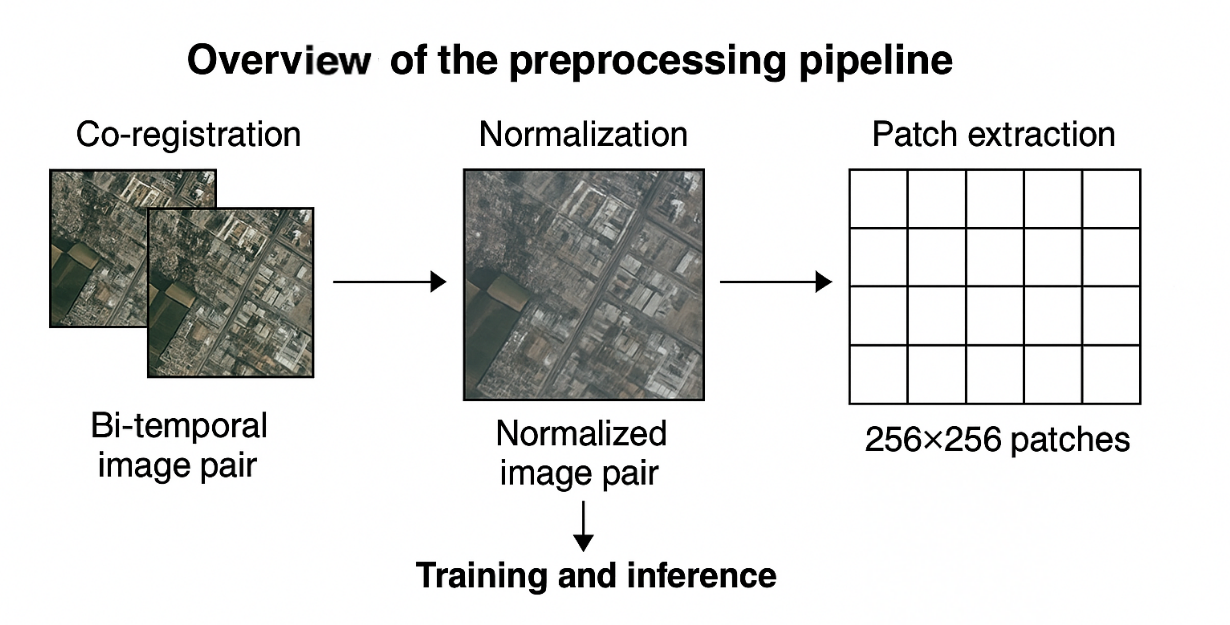
\includegraphics[width=0.6\textwidth]{graficos/Preprocessing.png}
    \caption{\textbf{Overview of preprocessing.} Bi-temporal pairs undergo co-registration, 
    normalization, and patch extraction, following the ChangeFormer protocol.}
    \label{fig:preprocessing}
\end{figure}



\section{Detection of Building Changes}
\label{sec:detection}

\noindent
The proposed method extends the \textbf{ChangeFormer} architecture 
\cite{Bandara2022ChangeFormer} by replacing its Multi-Head Self-Attention (MHSA) modules 
with the more efficient \textbf{Rank-Augmented Linear Attention (RALA)} 
\cite{Fan2025RALA}. The resulting model, denoted \textbf{RALA-ChangeFormer}, retains the 
hierarchical Siamese encoder–decoder design while reducing the computational cost of 
self-attention from quadratic to linear in the number of tokens.

\noindent \textbf{Dual-stream encoder.} Two weight-sharing Transformer encoders extract multi-level feature maps from the pre-event \(I_t^1\) and post-event \(I_t^2\) images. Patch embeddings and hierarchical downsampling produce progressively coarser but semantically richer feature sequences.

\noindent \textbf{Feature interaction.} At multiple scales, corresponding features from both streams are combined through concatenation and difference operations, allowing the model to emphasize spatial–temporal discrepancies associated with structural changes.

\noindent \textbf{Decoder.} A lightweight multi-scale decoder progressively upsamples the fused features to predict a dense change probability map \(\hat{Y}\). A final sigmoid activation produces values in \([0,1]\).

\begin{figure}[h!]
    \centering
    
\includegraphics[width=1\textwidth]{graficos/ChangeFormer.png}
    \vspace{0.4em}
    \rule{0.92\textwidth}{0.35pt}
    \vspace{0.4em}
    
\includegraphics[width=0.6\textwidth]{graficos/RALA.png}
    \caption{\textbf{Overview of the RALA-ChangeFormer architecture.} 
    The ChangeFormer encoder–decoder structure is retained, while MHSA layers are replaced by 
    the linear, rank-augmented RALA attention mechanism.}
    \label{fig:changeformer-arch}
\end{figure}



\newpage

\subsection{Integration of RALA into Transformer Blocks}
\label{subsec:rala-integration}

\noindent
Standard attention requires computing the similarity matrix 
\(QK^\top \in \mathbb{R}^{N\times N}\), which incurs quadratic complexity. 
RALA replaces this operation with a linear, kernel-based formulation that explicitly prevents 
rank collapse in both key–value aggregation and output features.

\paragraph{Kernel linearization.}
RALA begins by applying a positive feature map 
\(\kappa : \mathbb{R}^d \rightarrow \mathbb{R}^{d'}\) to queries and keys, rewriting attention as:
\[
\mathrm{Attn}_{lin}(Q,K,V)
=
\kappa(Q)\Big( \sum_{j=1}^N \kappa(K_j)^\top V_j \Big).
\]
This avoids constructing the \(N\times N\) matrix and reduces complexity to \(O(Nd)\).  
However, the matrix
\[
B_{lin} = \sum_{j=1}^N \kappa(K_j)^\top V_j
\]
is often low-rank, degrading dense prediction performance.

\paragraph{Rank augmentation (RALA).}
To mitigate rank collapse, RALA reweights each key–value contribution using token-dependent 
coefficients:
\[
B = \sum_{j=1}^N \alpha_j\, \kappa(K_j)^\top V_j,
\]
where the weights \(\alpha_j\) are derived from a global query:
\[
Q_g = \frac{1}{N}\sum_{i=1}^N Q_i,
\quad
\alpha_j 
=
N\,
\frac{\exp\!\big( \kappa(Q_g)\kappa(K_j)^\top \big)}
     {\sum_{m=1}^N \exp\!\big( \kappa(Q_g)\kappa(K_m)^\top \big)}.
\]
This increases the diversity of the aggregated components, restoring the effective rank of \(B\).

\paragraph{Output feature modulation.}
Even with a rank-augmented buffer, 
\(Y_i = \kappa(Q_i) B\)  
can remain low-rank because it lies within the span of \(\kappa(Q)\).
RALA introduces token-specific modulation:
\[
Y_i
=
\phi(X_i)
\odot 
\big(\kappa(Q_i) B\big),
\]
where \(\phi(\cdot)\) is a learned projection and \(\odot\) denotes elementwise multiplication.  
This restores output rank without increasing computational complexity.

\paragraph{Final RALA formulation.}
\[
B = \sum_{j=1}^N \alpha_j \kappa(K_j)^\top V_j,
\qquad
Y_i = \phi(X_i) \odot \big(\kappa(Q_i) B\big).
\]

\paragraph{Replacing MHSA.}
Each MHSA block in ChangeFormer is replaced with a RALA block, while residual connections, 
layer normalization, and feed-forward networks remain unchanged. This yields:
- linear complexity in sequence length,  
- full parallelization (no recurrence),  
- compatibility with the original architecture,  
- substantially reduced memory footprint.


\subsection{Loss Function and Training Objective}

\noindent
The model is trained using a hybrid loss combining Binary Cross-Entropy and Dice loss:
\[
\mathcal{L}
=
\mathcal{L}_{BCE}(Y,\hat{Y})
+
\mathcal{L}_{Dice}(Y,\hat{Y}),
\]
with
\[
\mathcal{L}_{Dice}
=
1
- 
\frac{2\sum_i Y_i\hat{Y}_i}
       {\sum_i Y_i + \sum_i \hat{Y}_i + \epsilon}.
\]
This formulation addresses pixel-wise accuracy and class imbalance simultaneously.

Training uses AdamW with a cosine learning rate schedule and warm-up epochs, following 
best practices for stable Transformer optimization.


\subsection{Inference and Change Classification}

\noindent
At inference time, the network predicts a dense probability map 
\(\hat{Y} \in [0,1]^{H\times W}\).  
A threshold \(\tau=0.5\) yields the final binary change mask:
\[
Y_{\text{bin}}(i,j)=
\begin{cases}
1, & \hat{Y}(i,j)\ge\tau,\\
0, & \text{otherwise}.
\end{cases}
\]
The resulting mask identifies building additions, removals, or structural modifications 
and serves as the input to the localization stage described in 
Section~\ref{sec:localization}.

\section{Localization of Building Changes}
\label{sec:localization}

\noindent
Once the model produces the probability map \(\hat{Y}\) from the detection stage, a final post-processing step is applied to obtain the explicit spatial localization of building changes. This process transforms the continuous probability predictions into a binary segmentation mask that highlights precise regions where construction, demolition, or structural modifications have occurred between two temporal images.

\medskip
\noindent
\textbf{(1) Binary Mask Generation.}  
The output of the RALA-ChangeFormer is a continuous-valued change probability map \(\hat{Y} \in [0,1]^{H\times W}\). Each pixel value represents the likelihood of a change occurring at that location. To convert this probabilistic representation into a discrete form, a thresholding operation is applied:
\[
M(i,j) = 
\begin{cases}
1, & \text{if } \hat{Y}(i,j) \geq \tau, \\
0, & \text{otherwise,}
\end{cases}
\]
where \(M\) denotes the binary change mask and \(\tau\) is an empirically chosen threshold. Consistent with prior work~\cite{Bandara2022ChangeFormer,Zheng2022HFANet}, we set \(\tau = 0.5\), which provides a balanced trade-off between precision and recall. Pixels with \(M(i,j)=1\) correspond to detected building changes, while \(M(i,j)=0\) indicates no change.

\medskip
\noindent
\textbf{(2) Morphological Refinement.}  
Although the model learns strong spatial correspondences, prediction noise may still produce small false positives or fragmented regions, especially near building edges. To mitigate this, morphological operations are applied to the binary mask:
\begin{itemize}
    \item \textbf{Erosion:} Removes isolated noise pixels, enhancing boundary sharpness.
    \item \textbf{Dilation:} Expands valid change regions to restore structural continuity after erosion.
    \item \textbf{Opening and Closing:} Sequentially applying erosion and dilation smooths the mask and consolidates fragmented regions.
\end{itemize}
These post-processing steps ensure that the resulting mask accurately aligns with building boundaries, improving the visual and quantitative quality of the final localization.

\medskip
\noindent
\textbf{(3) Multi-scale Fusion and Visualization.}  
For better interpretability, the localized change mask \(M\) is overlaid onto the original pre- and post-event images. Multi-scale fusion is performed by resizing the mask back to the original spatial resolution of the input imagery (\(1024\times1024\) for LEVIR-CD and \(512\times512\) for DSIFN-CD). This enables intuitive visualization of building additions and removals within their geographic context.

\begin{figure}[h!]
    \centering
    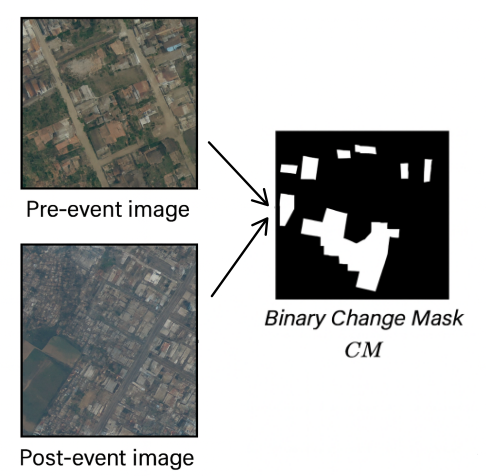
\includegraphics[width=0.6\textwidth]{graficos/Localization_mask.png}
    \caption{\textbf{Localization of building changes.} The probability map produced by the RALA-ChangeFormer is thresholded (\(\tau=0.5\)) and refined with morphological operations to generate a binary mask highlighting changed building areas.}
    \label{fig:localization}
\end{figure}

\medskip
\noindent
\textbf{(4) Output Interpretation.}  
The localized binary masks serve as the final deliverable for both qualitative analysis and quantitative evaluation using metrics such as Intersection-over-Union (IoU) and F1-score. Each mask distinctly highlights building-level changes between temporal image pairs, enabling urban planners and remote sensing specialists to monitor construction dynamics, urban densification, and infrastructure evolution efficiently.

\medskip
\noindent
This localization stage completes the change detection pipeline by converting model outputs into interpretable spatial representations that can be directly utilized for mapping and decision-support applications.


\section{Final Considerations}
\label{sec:final-considerations}

\noindent
This chapter presented the complete design of the proposed \textbf{RALA-ChangeFormer} framework for building change detection from very-high-resolution satellite imagery. The proposed pipeline combines efficient Transformer-based feature extraction with precise spatial localization, balancing computational feasibility with high accuracy across urban scenarios.

\medskip
\noindent
The preprocessing stage ensured standardized input handling through co-registration, normalization, and patch extraction of \(256 \times 256\) non-overlapping samples from bi-temporal images. This strategy, supported by mild data augmentation, enhanced the diversity and representativeness of training samples drawn from LEVIR-CD and DSIFN-CD datasets, while maintaining spatial coherence.

\medskip
\noindent
At the core of the detection stage, the RALA-ChangeFormer integrates the \textbf{Recurrent Approximation Linear Attention (RALA)} mechanism into the Transformer encoder blocks of the \textbf{ChangeFormer} architecture~\cite{Bandara2022ChangeFormer, Fan2025RALA}. This modification allows the model to retain the global context awareness characteristic of Transformers while significantly reducing memory consumption and computational cost from quadratic to near-linear complexity. As a result, the model efficiently scales to large satellite patches without sacrificing representational quality.

\medskip
\noindent
The detection and classification process employed a hybrid loss function combining Binary Cross-Entropy and Dice losses to address class imbalance and boundary precision. During inference, a pixel-wise probability map was generated and thresholded at \(\tau=0.5\) to classify each pixel as \emph{change} or \emph{no-change}. This enabled accurate delineation of building-level transitions.

\medskip
\noindent
The localization stage refined the raw outputs through morphological operations, eliminating noise and consolidating fragmented regions to yield interpretable binary change masks. These masks were then fused with the original temporal images to visualize structural changes at the building scale, facilitating their application in urban growth monitoring, damage assessment, and land-use analysis.

\medskip
\noindent
In summary, the proposed architecture effectively integrates efficient linear attention into a Transformer-based Siamese framework, improving scalability and precision in building change detection. The RALA-ChangeFormer establishes a foundation for future work on \textbf{self-supervised or cross-domain transfer learning} in urban change analysis, aiming to further reduce dependence on labeled data while maintaining high localization accuracy.